\AtBeginSection[]{
    \begin{frame}
        \frametitle{}
        \tableofcontents[currentsection]
    \end{frame}
}

%%%%%%%%%%%%%%%%%%%%%%%%%%%%%%%%%%%%

\section{Theoretical background}

\subsection{Multi-Agent Systems context}

\begin{frame}[allowframebreaks]{Theoretical background}{Multi-Agent Systems context}

    \begin{block}{Keywords}
        \begin{itemize}
            \item \textbf{Agent}: entity immersed in an environment perceiving observation and making decision autonomously to achieve some goals;
            \item \textbf{MAS}: a set of agents collaborating with self/re-organizing mechanisms to achieve their goal;
            \item \textbf{Organization}: the agents' interactions even though it may be implicit;
            \item \textbf{Organizational Model}: used as a medium to describe an explicit/implicit known organization;
            \item \textbf{Organizational Specifications}: the components used in an organizational model to characterize the organization
        \end{itemize}
    \end{block}

    \begin{block}{Organizational model: $\mathcal{M}OISE^+$}
        \begin{itemize}
            \item possible to link agents' policies to organizational specifications
            \item takes into account the social aspects between agents explicitly (whereas \emph{AGR} focuses on the integration of standards oriented towards design)
        \end{itemize}
    \end{block}

    


\tikzset{every picture/.style={line width=0.75pt}} %set default line width to 0.75pt        

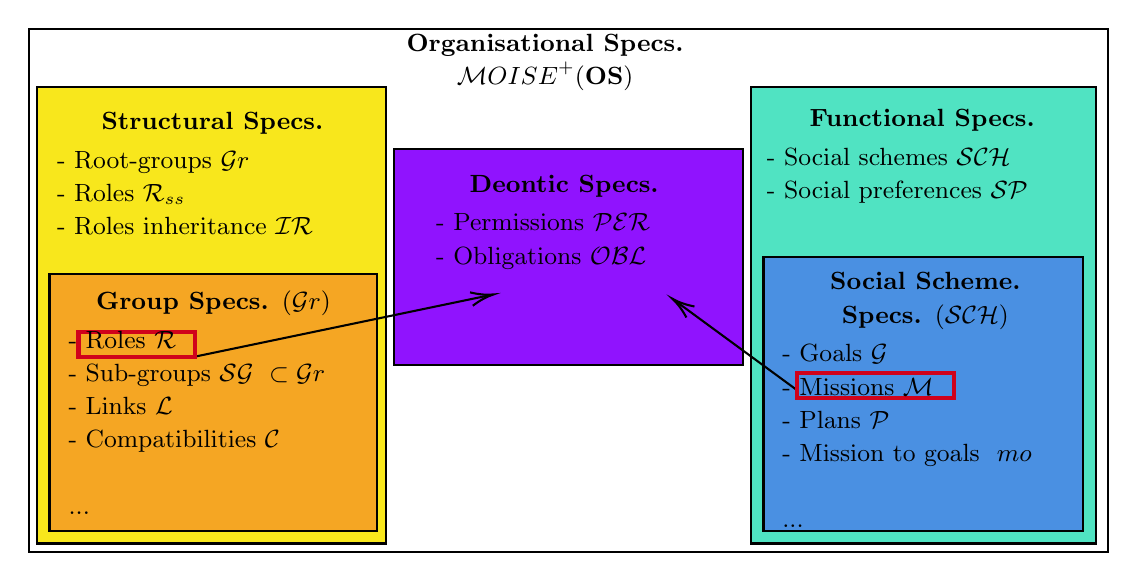
\begin{tikzpicture}[x=0.75pt,y=0.75pt,yscale=-1,xscale=1]
%uncomment if require: \path (0,1656); %set diagram left start at 0, and has height of 1656

%Shape: Rectangle [id:dp6756844921493015] 
\draw  [fill={rgb, 255:red, 248; green, 231; blue, 28 }  ,fill opacity=1 ] (46,1204) -- (214,1204) -- (214,1424) -- (46,1424) -- cycle ;
%Shape: Rectangle [id:dp3759944257810566] 
\draw  [fill={rgb, 255:red, 80; green, 227; blue, 194 }  ,fill opacity=1 ] (390,1204) -- (556,1204) -- (556,1424) -- (390,1424) -- cycle ;
%Shape: Rectangle [id:dp28244406216006945] 
\draw  [fill={rgb, 255:red, 144; green, 19; blue, 254 }  ,fill opacity=1 ] (218,1234) -- (386,1234) -- (386,1338) -- (218,1338) -- cycle ;
%Shape: Rectangle [id:dp32232123359581766] 
\draw   (42,1176) -- (562,1176) -- (562,1428) -- (42,1428) -- cycle ;
%Shape: Rectangle [id:dp7605706269262755] 
\draw  [fill={rgb, 255:red, 74; green, 144; blue, 226 }  ,fill opacity=1 ] (396,1286) -- (550,1286) -- (550,1418) -- (396,1418) -- cycle ;
%Shape: Rectangle [id:dp33110985390647496] 
\draw   (52,1294) -- (210,1294) -- (210,1418) -- (52,1418) -- cycle ;
%Shape: Rectangle [id:dp8653560038381976] 
\draw  [fill={rgb, 255:red, 245; green, 166; blue, 35 }  ,fill opacity=1 ] (52,1294) -- (210,1294) -- (210,1418) -- (52,1418) -- cycle ;
%Straight Lines [id:da09781093164567278] 
\draw    (412,1350) -- (353.61,1307.18) ;
\draw [shift={(352,1306)}, rotate = 36.25] [color={rgb, 255:red, 0; green, 0; blue, 0 }  ][line width=0.75]    (10.93,-3.29) .. controls (6.95,-1.4) and (3.31,-0.3) .. (0,0) .. controls (3.31,0.3) and (6.95,1.4) .. (10.93,3.29)   ;
%Straight Lines [id:da3938396723807833] 
\draw    (122,1334) -- (264.04,1304.41) ;
\draw [shift={(266,1304)}, rotate = 168.23] [color={rgb, 255:red, 0; green, 0; blue, 0 }  ][line width=0.75]    (10.93,-3.29) .. controls (6.95,-1.4) and (3.31,-0.3) .. (0,0) .. controls (3.31,0.3) and (6.95,1.4) .. (10.93,3.29)   ;
%Shape: Rectangle [id:dp269311335478327] 
\draw  [color={rgb, 255:red, 208; green, 2; blue, 27 }  ,draw opacity=1 ][line width=1.5]  (66,1322) -- (122,1322) -- (122,1334) -- (66,1334) -- cycle ;
%Shape: Rectangle [id:dp7449860119164387] 
\draw  [color={rgb, 255:red, 208; green, 2; blue, 27 }  ,draw opacity=1 ][line width=1.5]  (412,1342) -- (488,1342) -- (488,1354) -- (412,1354) -- cycle ;


% Text Node
\draw (472.5,1237.41) node   [align=left] {\begin{minipage}[lt]{112.2pt}\setlength\topsep{0pt}
\begin{center}
\textbf{{\small Functional Specs.}}
\end{center}
{\small  - Social schemes $\displaystyle \mathcal{SCH}$}\\{\small  - Social preferences $\displaystyle \mathcal{SP}$}
\end{minipage}};
% Text Node
\draw (474,1355) node   [align=left] {\begin{minipage}[lt]{103.36pt}\setlength\topsep{0pt}
\begin{center}
\textbf{{\small Social Scheme.}}\\{\small \textbf{Specs. }$\displaystyle (\mathcal{SCH})$}
\end{center}
{\small  - Goals $\displaystyle \mathcal{G}$}\\{\small  - Missions $\displaystyle \mathcal{M}$}\\{\small  - Plans $\displaystyle \mathcal{P}$}\\{\small  - Mission to goals \ $\displaystyle mo$}\\\\{\small  ...}
\end{minipage}};
% Text Node
\draw (131,1356) node   [align=left] {\begin{minipage}[lt]{104.72pt}\setlength\topsep{0pt}
\begin{center}
{\small \textbf{Group Specs. }$\displaystyle (\mathcal{G} r)$}
\end{center}
{\small  - Roles $\displaystyle \mathcal{R}$}\\{\small  - Sub-groups $\displaystyle \mathcal{SG} \ \subset \mathcal{G} r$}\\{\small  - Links $\displaystyle \mathcal{L}$}\\{\small  - Compatibilities $\displaystyle \mathcal{C}$}\\\\{\small  ...}
\end{minipage}};
% Text Node
\draw (181,1177) node [anchor=north west][inner sep=0.75pt]   [align=left] {\begin{minipage}[lt]{162.41pt}\setlength\topsep{0pt}
\begin{center}
{\small \textbf{Organisational Specs. }$\displaystyle \mathcal{M}\boldsymbol{OISE^{+}}$($\displaystyle \mathbf{OS}$)}
\end{center}

\end{minipage}};
% Text Node
\draw (300,1269.09) node   [align=left] {\begin{minipage}[lt]{92.48pt}\setlength\topsep{0pt}
\begin{center}
\textbf{{\small Deontic Specs.}}
\end{center}
{\small  - Permissions $\displaystyle \mathcal{PER}$}\\{\small  - Obligations $\displaystyle \mathcal{OBL}$}
\end{minipage}};
% Text Node
\draw (130.5,1245.69) node   [align=left] {\begin{minipage}[lt]{112.2pt}\setlength\topsep{0pt}
\begin{center}
\textbf{{\small Structural Specs.}}
\end{center}
{\small  - Root-groups $\displaystyle \mathcal{G} r$}\\{\small  - Roles $\displaystyle \mathcal{R}_{ss}$}\\{\small  - Roles inheritance $\displaystyle \mathcal{IR}$}
\end{minipage}};


\end{tikzpicture}

\end{frame}


\subsection{MARL basics}

\begin{frame}[allowframebreaks]{Theoretical background}{MARL basics}

    \begin{block}{Keywords}
        \begin{itemize}
            \item \textbf{Policy}: the \textquote{logic} to choose next action according to observation for an agent;
            \item \textbf{History/trajectory}: the tuple of (observation, action) couples over an episode;
            \item \textbf{Joint-policy / Joint-history}: all of the agents' policies / histories as tuples;
            \item \textbf{Reinforcement learning}: an agent updates its policy to maximize a cumulative reward;
            \item \textbf{Multi-Agent Reinforcement Learning (MARL)}: extends to multiple agents that learn while considering the actions of other agents;
        \end{itemize}
    \end{block}

    \begin{block}{MARL for methodological purpose}

        Effective joint-policies but not explicitly specified/understandable
        $\Longrightarrow$ Few related works

        \begin{itemize}
            \item Kazhdan et. al.~\cite{Kazhdan2020} proposed means to extract symbolic models;
            \item Wang et. al.~\cite{Wang2020}: introduced a role-oriented MARL approach;
            \item Zheng et. al.~\cite{Zheng2018} presented a platform for MARL.
        \end{itemize}
    \end{block}

    \begin{block}{Markovian models for MARL: Dec-POMDP}
        Decentralized Partially Observable Markov Decision Process~\cite{Oliehoek2016}
        \begin{itemize}
            \item considers multiple agents in a similar MAS fashion
            \item stochastic processes for uncertainty in environmental changes including observations;
            \item reward function is common to agents which fosters training for collaborative oriented actions~\cite{Beynier2013}
        \end{itemize}

        \

        { \footnotesize

        $(S,\{A_i\},T,R,\{\Omega_i\},O,\gamma)$ , where
        \begin{itemize}
            \item $S = \{s_1, ..s_{|S|}\}$: The set of the possible states;
            \item $A_{i} = \{a_{1}^{i},..,a_{|A_{i}|}^{i}\}$: The set of the possible actions for agent $i$;
            \item $T$ so that $T(s,a,s') = \probP{(s'|s,a)}$ : The set of conditional transition probabilities between states;
            \item $R: S \times A \times S \rightarrow \mathbb{R}$: The reward function
            \item $\Omega_{i} = \{o_{1}^{i},..,o_{|\Omega_{i}|}^{i}\}$: The set of observations for agent $ag_i$;
            \item $O$ so that $O(s',a,o) = \probP{(o|s',a)}$ : The set of conditional observation probabilities;
            \item $\gamma \in [0,1]$, the discount factor.
        \end{itemize}

        }

    \end{block}

    \begin{block}{Solving a Dec-POMDP}
        \begin{itemize}
            \item \textbf{solving} the Dec-POMDP for the team $t$ as finding a joint policy $\pi_{joint,i} \in \Pi_{joint}$ that maximizes the expected cumulative reward over a finite horizon;
            \item \textbf{sub-optimally solving} the Dec-POMDP at $s$ expectancy as finding the joint policies $\pi_{joint,i} \in \Pi_{joint}$ that gets the expected cumulative reward over a finite horizon at least at $s \in \mathbb{R}$.
        \end{itemize}
    \end{block}

    \begin{exampleblock}{Examples of MARL Algorithms}
        \begin{itemize}
            \item \textbf{Independent Learning}: IQL, IDQN
            \item \textbf{Centralized Training, Decentralized Execution}: MADDPG, COMA, VDN
            \item \textbf{Cooperative MARL}: QMIX, MAPPO
            \item \textbf{Hierarchical MARL}: Feudal Networks, Hierarchical Actor-Critic
            \item \dots
        \end{itemize}
    \end{exampleblock}

\end{frame}
